%!TEX root = ../main.tex
\chapter{Implementácia aplikácie}
Táto kapitola rozoberá spôsoby akými boli implementované riešenia problémov. Popisuje prečo boli vybrané práve použité platformy,

\section{Výber platformy}
Vytváraný framework je založený na klient-server architektúre. Bolo preto potrebné vybrať najvhodnejšie platformy na implementáciu pre obe časti.
\subsection{Klient}
Trebalo brať v úvahu, že zariadenie, na ktorom pôjde herný klient, bude potrebovať GPS senzor a bude musieť byť mobilné. Preto boli vybrané platformy, ktoré sa vyskytujú práve na mobilných zariadeniach s pripojením na internet a so senzormi. Možnosti teda boli Android, iOS, Windows Phone 8, poprípade vyvíjať multiplatformovo pomocou riešení ako sú Xamarin, Phonegap či Appcelerator. Na prvý pohľad by bol najlepším riešením vývoj pre viaceré platformy naraz. Pri lepšom pohľade je ale jasné, že v konečnom dôsledku je potrebné upravovať program pre jednotlivé platformy, kvôli ich odlišnostiam. Vzniká teda otázka, na ktorú platformu sa sústrediť. Android platforma pre svoju rozšírenosť (väčší podiel na trhu oproti Windows Phone) a dostupnosť (cenová oproti iOS) vyhráva oproti konkurentom a preto bola vybraná. Ostatné platformy by však nemali byť zanedbané a mali by byť predmetom budúcich rozširovaní frameworku. 


\subsection{Server}
Linuxová platforma bola vybraná nielen pre cenu, stabilitu a bezpečnosť, no hlavne jej rozšírenosť u hostingových služieb. Kvôli tomu bolo riešenie pomocou ASP.NET zavrhnuté. Ďalšími zvažovanými možnosťami boli frameworky ako Ruby on Rails, NodeJs a CodeIgniter. Každý z nich funguje v inom prostredí. Prvé dva sú veľmi progresívne a silné frameworky. Pomocou jazyka Ruby v Rails frameworku možno vytvoriť veľmi rýchlo generickú aplikáciu na manažment obsahu. Určitou výhodou a zároveň aj nevýhodou sú silno presadzované spôsoby ako programovať v Rails, ktoré dokážu veľmi urýchliť vývoj aplikácii, ale aj spomaliť pri drobnostiach. NodeJs je veľmi dobrý pri zvládaní konkurentných požiadaviek, a lákavý tiež pre svoju rýchlosť a spracovávanie udalostí. Nakoniec bol však vybraný Code Igniter napísaný v jazyku PHP, pre moje skúsenosti s týmto jazykom a bežnosťou jeho podpory u hostingových služieb.


\section{Vývojové prostredie}
Pri vyvíjaní klientskej aplikácie bol využitý program Android Studio, ktorý je špecializovaný na vývoj aplikácii pre platformu Android. Na vývoj serverovej aplikácie bol použitý Sublime Text 3. Ako verzionovací systém bol použitý Git na službe GitHub.

\section{Dôležité triedy a ich popis}
\subsection{Klient}
\subsubsection{Komunikácia s online API}
Na komunikáciu slúži trieda \emph{MyHTMLBrowser}, ktorá sa stará o posielanie POST a GET žiadostí na server. Trieda je naprogramovaná pomocou návrhového vzoru singleton, pre lepšiu perzistenciu dát. Trieda ponúka množstvo verejných metód:
\begin{itemize}
  \item \emph{getInstance(Context context)} - metóda z návrhového vzoru singleton, pre vrátenie existujúcej inštancie \emph{MyHTMLBrowser} poprípade jej vytvorenia
  \item \emph{isOnline()} - metóda zistí či je zariadenie pripojené k sieti internet 
\end{itemize}

\paragraph*{Všeobecné požiadavky} vrátia textový reťazec. 
\begin{itemize}
  \item \emph{HttpGetString(String url)} - navštívi \emph{url} webovej stránky a vráti jej obsah ako textový reťazec.
  \item \emph{HttpPostString(String url, List<NameValuePair> nameValuePairs)} - pošle Post požiadavku na zadanú \emph{url} s premennými, ktoré sa nachádzajú v \emph{nameValuePairs}. 
  \item \emph{HttpGetAsyncString(Context context, String url, AsyncResponse delegate)} - asynchrónna metóda, ktorá môže byť spustená z hlavného vlákna. \emph{AsyncResponse} je interface, ktorému možno prepísať metódu \emph{processFinish(Context context, String output)}, ktorá je volaná po získaní textového reťazca zo stránky.  
  \item \emph{HttpPostAsyncString(Context context, String url, List<NameValuePair> postPairs, AsyncResponse delegate)} - oproti asynchrónnej GET metóde pribudol parameter s POST premennými. 
\end{itemize}



\paragraph*{Špecifické požiadavky} sú uspôsobené už s presne zadaným formátom požiadavky. Vrátia objekt \emph{Response}.
\begin{itemize}
  \item \emph{Login(String user, String pass, String serverURL)} - metóda využívaná na prihlasovacej obrazovke, posiela Post požiadavok na danú \emph{serverURL}. S pridaním časti adresy pre API metódu prihlásenia.
  \item \emph{Register(String user, String pass, String serverURL)} - má rovnaké parametre ako \emph{Login} a slúži na vytvorenie nového používateľa pomocou serverovej API. 
\end{itemize}

\subsubsection{Konverzia JSON a trieda Response}
Po úspešnej komunikácii klienta s hernou API klient dostáva textovú odpoveď vo formáte JSON. Táto informácia je spracovaná triedou \emph{ResponseJSONParser}, ktorá má statické metódy
\begin{itemize}
   \item \emph{parseGameData(String json)} vráti GameData objekt, ktorý obsahuje polia s objektami regiónov, objektov, atribútov, úloh či odpovedí.
  \item \emph{getQuestFromJSONObj(JSONObject jsonQuestObj)}
   \item \emph{getRegionFromJSONObj(JSONObject jsonRegionObj)}
   \item \emph{getItemFromJSONObj(JSONObject itemJsonObj)}
   \item \emph{getAttributeJSONObj(JSONObject attributeJsonObj)}
   \item \emph{parseResponse(String json)} vráti h
\end{itemize}


\paragraph*{Response} je trieda, ktorá vzniká iba spracovaním JSON odpovedí z herného serveru. Preto jej konštruktor dostáva ako parameter JSON reťazec obsahujúci \emph{JSONObject}, ktorý je spracovaný pomocou metódy parseJson na tieto časti: \emph{type} - popisuje o aký typ odpovede sa jedná, podľa ktorého je spracovaná. \emph{Success} - informuje o tom, či bola odpoveď úspešná. \emph{Message} - obsahuje textový reťazec, ktorý je väčšinou zobrazovaný používateľovi ako odozva na požiadavku. \emph{Data} - je triedy \emph{Object} a môže obsahovať objekt z rôznych tried v závislosti na type odpovede. Podľa toho o aký typ odpovede sa jedná je premenná ďalej spracovaná. Napríklad pri type odpovede, ktorý špecifikuje prijatie úlohy \emph{data} reťazec obsahuje JSON objekt s prijatou úlohou.

\lstset{language=Java,
basicstyle=\tiny
}        
\begin{lstlisting}[frame=single]
 private void parseJson(String json) {
        if (json != null && !json.isEmpty()) {
            try {
                JSONObject jsonResponseObj = new JSONObject(json);
                type = jsonResponseObj.optString(KEY_TYPE, "");
                success = jsonResponseObj.optString(KEY_SUCCESS, "0").equals("1");
                message = jsonResponseObj.optString(KEY_MESSAGE, "");
                dataString = jsonResponseObj.optString(KEY_DATA, "");
                Log.d(TAG, dataString);
                if (type.equals(TYPE_IS_LOGGED)) {
                    loggedOut = !success;
                }
                if (!dataString.equals("")) data = getDataFromResponse(dataString, type);
                successfullyParsed = true;
            } catch (JSONException e) {
                e.printStackTrace();
                successfullyParsed = false;
            }
        } else {
            Log.e(TAG, "No json string to parse");
        }
        successfullyParsed = false;
    }
\end{lstlisting}

\subsection{Server}
\subsubsection{Cron}
Aby sa mohli regióny pohybovať bolo potrebné spustiť službu \emph{Cron}, ktorá má na starosti spúšťanie skriptov v určitom čase alebo časovom intervale. Používateľ môže pri tvorbe/úprave regiónu nastaviť jeho pohyb a meniť jeho hranice pomocou mapy. Pomocou tlačidla na pridanie nového bodu pohybu sa po zmene vlastností regiónu uložia to JSON pola. Výsledný pohyb je možný prehrať na mape. Toto pole sa uloží do tabuľky, ktorá je neskôr dopytovaná skriptom, ktorý je spustený \emph{Cronom}. Zápisy, ktoré dopyt získa sú spracované a zmeny vlastností regiónov sú vykonané pomocou verejnej metódy \emph{(\$name, \$info, \$image, \$lat\_start, \$lon\_start, \$lat\_end, \$lon\_end, \$movement)} modelu \emph{Region\_m}.

% \lstset{language=PHP,
% basicstyle=\tiny}          % Set your language (you can change the language for each code-block optionally)

% \begin{lstlisting}[frame=single]  % Start your code-block

% \end{lstlisting}

\section{QR kódy}
\subsection{Generovanie}
O generovanie QR kódov sa stará knižnica PHP QR Code. Tá musela byť upravená pre Code Igniter. Knižnica však nepodporovala možnosť ďalších úprav vygenerovaného obrázku QR kódu. Tieto úpravy boli potrebné pre možnosť automatického pridávanie loga hry na obrázok. Jedna z možností bola obrázok uložiť na disku a znovu načítať a upraviť. Tá bola však hneď na prvý pohľad zlá, pre jej náročnosť na disk a iné zdroje. Preto bola potrebná úprava tejto knižnice. Boli implementované funkcie, ktoré vrátia obrázok ako upravovateľný zdroj. Bola teda využitá jedna z metód, ktorá vracia vygenerovaný QR kód ako dvojrozmerné pole jednotiek a núl (symbolizujúcich čierne a biele políčka). Toto pole -\emph{\$frame}  je posielané ako jeden z parametrov do novovytvorenej funkcie, ktorá žiadaný obrázok generuje. \

\lstset{language=PHP,
basicstyle=\tiny}
\begin{lstlisting}[frame=single]  % Start your code-block
        public static function image($frame, $pixelPerPoint = 4, $outerFrame = 4) 
        {
            $h = count($frame);
            $w = strlen($frame[0]);
            
            $imgW = $w + 2*$outerFrame;
            $imgH = $h + 2*$outerFrame;
            
            $base_image =ImageCreate($imgW, $imgH);
            
            $col[0] = ImageColorAllocate($base_image,QRImage::$black[0],
            				QRImage::$black[1],QRImage::$black[2]);
            $col[1] = ImageColorAllocate($base_image,QRImage::$white[0],
           				QRImage::$white[1],QRImage::$white[2]);

            imagefill($base_image, 0, 0, $col[0]);

            for($y=0; $y<$h; $y++) {
                for($x=0; $x<$w; $x++) {
                    if ($frame[$y][$x] == '1') {
                        ImageSetPixel($base_image,$x+$outerFrame,$y+$outerFrame,$col[1]); 
                    }
                }
            }
            
            $target_image = ImageCreate($imgW * $pixelPerPoint, $imgH * $pixelPerPoint);
            ImageCopyResized($target_image, $base_image, 0, 0, 0, 0, $imgW * $pixelPerPoint, 
            					$imgH * $pixelPerPoint, $imgW, $imgH);
            ImageDestroy($base_image);
            
            return $target_image;
        }
\end{lstlisting}


\subsection{Čítanie}
O čítanie sa stará aktivita \emph{ScannerActivity}, ktorá implementuje \emph{ZBarScannerView.ResultHandler}. Ten ponúka metódu na prepísanie \emph{handleResult(Result rawResult)}, v ktorej je jej parameter spracovaný. Kód, ktorý sa získa, je automaticky poslaný na herný server na overenie jeho existencie a zistenie informácii o ňom. Server na tento požiadavok pošle odpoveď (\emph{Response}), ktorú klient spracuje a podľa toho zobrazí potrebné obrazovky alebo správu.


\section{Bluetooth}
O komunikáciu medzi zariadeniami pomocou Bluetooth technológie sa stará trieda \emph{BTCommunicator}. Tá obsahuje tri triedy, ktoré dedia od vlákien. Pomocou nich je vytvorená klient-server architektúra.
\begin{itemize}
	\item \emph{AcceptThread} - správa sa ako serverový komponent a očakáva pripojenia od klientov
    \item \emph{ConnectThread} - toto vlákno nadväzuje pripojenie z klientskej strany 
    \item \emph{ConnectedThread} - po úspešnom pripojením beží práve toto vlákno, ktoré pomocou metód \emph{getInputStream()} a \emph{getOutputStream()} získa objekty tried \emph{InputStream} a \emph{OutputStream}. Tie umožňujú komunikáciu medzi zariadeniami a posielajú si navzájom polia bytov.
\end{itemize}

% \section{Mapy}
% V jednom z fragmentom, je použitá mapa. Tento komponent z 
% AAAAAAAAAAAAAAAAAAAAAAAAAAAAAAAAAAAAAAAAAAAAAAAAAAAAAAAAAAAAAAAAAAAAAAAAAAAAAAAAAAAAAAAAAAAAAAAAAAAAAAAAAAAAAAAAAAAAA

\section{Synchronizácia súborov}
Jednostranná synchronizácia klienta a herného serveru zaručuje, aby klient obsahoval všetky potrebné obrázky, ktoré by na ňom mohli chýbať. Túto synchronizáciu je možné nastaviť v nastaveniach ako automatickú (pri úspešnom prihlásení sa na server). Pomocou tlačidla synchronizácie je ju možné vyvolať manuálne. Klient ako prvé, zistí zoznam obrázkov, ktoré má v hernej zložke na klientovi. Tento zoznam porovná so zoznamom, ktorý dostal z požiadavky na serverové API. Ak na serveri pribudli obrázky, klient to zistí jednoduchým porovnaním týchto zoznamov a chýbajúce obrázky stiahne.


\section{Zisťovanie aktuálnej polohy}
Na zisťovanie aktuálnej polohy slúži servis, ktorý sa snaží zistiť polohu pomocou GPS senzora, poprípade internetovej siete, ku ktorej je pripojený. Trieda \emph{GPSTracker} implementuje listener OnLocationChanged, pomocou ktorého je trieda notifikovaná o zmene polohy. V nastaveniach je možné nastaviť, aká je minimálna vzdialenosť a časový odstup v sekundách pre spustenie tejto metódy. Nachádza sa tu aj voľba vypnúť toto automatické zisťovanie polohy. 
\lstset{language=Java,
basicstyle=\tiny}
\begin{lstlisting}[frame=single]   
   public void onLocationChanged(final Location location) {
        this.location = location;
        latitude = location.getLatitude();
        longitude = location.getLongitude();
        String url = shade.pixel.gpsoclient.Settings.getUrlUpdatePosition(latitude,longitude);
        htmlBrowser = MyHtmlBrowser.getInstance(mContext);
        htmlBrowser.HttpGetAsyncString(mContext, url, new AsyncResponse() {
            @Override
            public void processFinish(Context context, String json) {
                Response response = new Response(json);
                if (response.isLoggedOut()) {
                    StartLoginActivity();
                } else {
                    GameData gameData = ResponseJSONParser.parseGameData(json);
                    GameHandler.gameHandler.setGameData(gameData);
                    if (gameData != null) {
                        if(mActivity!=null) { 
                            mActivity.SetQuestsView();
                            mActivity.SetRegionsView();
                            mActivity.SetItemsView();
                            mActivity.SetAttributesView();
                            mActivity.showResponses();
                        }
                    } else {
                        Log.d(TAG, "Problem with parsing gamedata");
                    }
                }
            }
        });
    }
\end{lstlisting}



\section{Databáza}
\subsection{Trieda modelu}
Databáza MySQL, ktorú aplikácia využíva, komunikuje s Code Igniter frameworkom fungujúcim na PHP. Ten pracuje s jednotlivými dátami z databáz pomocou triedy \emph{Active Record}. O získavanie dát z databázy sa starajú triedy, ktoré dedia od \emph{MY\_Model}, ktorá dedí od Code Igniter triedy \emph{CI\_Model}. \emph{MY\_Model} má mnohé protected premenné, ktoré popisujú vlastnosti tabuliek ako sú napríklad: názov, primárny kľúč, zoraďovanie zápisov, či pravidlá, ktoré musia jednotlivé vstupy spĺňať, aby boli zapísané do tabuľky. Tie sú upravené podľa potrieb jednotlivých modelov, ktoré od neho zdedili. Ďalej obsahuje množstvo verejných metód. 
\begin{itemize}
 \item \emph{array\_from\_post(\$fields)} vytvára podľa poľa \emph{\$fields} s názvami premenných, z POST požiadavky pole s rovnomennými kľúčmi, potom ako prešlo kontrolou validity pravidiel daného modelu.  Neskôr môže byť toto pole poslané metóde
 \item \emph{save(\$data, \$id = NULL)} - vytvára nový zápis do tabuľky, pokiaľ nie je zadaný primárny kľúč. Ak by parameter \emph{\$id} zadaný bol, tak metóda iba upraví existujúci zápis. 
 \item Metóda {delete(\$id)} vymaže zápis so zadaným primárnym kľúčom. 
 \item Na získavanie zápisov v tabuľke slúži \emph{get(\$id = NULL, \$single = FALSE)}, ktorá má dva parametre. Ak je zadaný parameter \emph{\$id}, tak funkcia vráti konkrétny zápis so zhodným primárnym kľúčom. Ak zadaný nie je a druhý parameter je pravdivý tak vráti jeden zápis, ináč vráti všetky z tabuľky.
 \item \emph{get\_array(\$id = NULL, \$single = FALSE)}, sa správa podobne ako predchádzajúca metóda, ale výsledok dopytu vráti ako pole, ktoré obsahuje polia s kľúčmi identickými k názvom premenných získaných objektov. 
 \item Funkcia \emph{get\_by(\$where, \$single = FALSE)} vyhľadá podľa parametru \emph{\$where} zápisy, ktoré ho spĺňajú. Ak je pravdivý parameter \emph{\$single}, funkcia vráti iba jeden zápis. Rovnako sa správa funkcia \emph{get\_array\_by(\$where, \$single = FALSE)}, ktorá tak, ako v predchádzajúcom prípade vráti, zápisy ako polia. 
\item Často používaná funkcia \emph{get\_by\_id(\$id)}, ktorá zistí, či existuje zápis so zadaným primárnym kľúčom.
\end{itemize}


 % \emph{array\_from\_post(\$fields)} vytvára podľa poľa \emph{\$fields} s názvami premenných z POST požiadavky pole s rovnomennými kľúčmi, potom ako prešlo kontrolou validity pravidiel daného modelu.  Neskôr može byť toto pole poslané metóde \emph{save(\$data, \$id = NULL)}, ktorá vytvorí nový zápis do tabuľky pokiaľ nie je zadaný primárny klúč. Ak by parameter \emph{\$id} zadaný bol, tak bude metóda upraví existujúci zápis. Metóda {delete(\$id)} vymaže zápis so zadaným primárným kľúčom. Táto trieda má tiež rôzne funkcie, na získavanie zápisov v tabuľke: \emph{get(\$id = NULL, \$single = FALSE)}, \emph{get\_array(\$id = NULL, \$single = FALSE)}, sa správa podobne ako predchádzajúca metóda ale výsledok dopytu vráti ako pole, ktoré obsahuje polia s kľúčmi identickými k názvom premenných získaných objektov. Funkcia \emph{get\_by(\$where, \$single = FALSE)} vyhladá podľa parametru \emph{\$where} zápisy, poprípade iba jeden, ak je nastavený parameter \emph{\$single}. Rovnako sa správa funkcia \emph{get\_array\_by(\$where, \$single = FALSE)}, ktorá tak ako v predchádzajúcom prípade vráti zápisy ako polia. Nachádza sa tu tiež často používaná funkcia \emph{get\_by\_id(\$id)}, ktorá zisťí, či existuje zápis so zadaným primárnym kľúčom.

\lstset{language=PHP,
basicstyle=\tiny}
\begin{lstlisting}[frame=single]
	public function get($id = NULL, $single = FALSE){
		if($id != NULL){
			$filter = $this->_primary_filter;
			$id = $filter($id);
			$this->db->where($this->_primary_key, $id);
			$method = 'row';
		} elseif($single == TRUE){
			$method = 'row';
		} else {
			$method = 'result';
		}
		if(!count($this->db->ar_orderby)){
			$this->db->order_by($this->_order_by);
		}
		return $this->db->get($this->_table_name)->$method();
	}
\end{lstlisting}

\subsection{Štruktúra tabuliek}
Pomocou migrácii boli k modelom vytvorené tabuľky, s ktorými manipulujú. 

\begin{figure}[h]
  \centering
   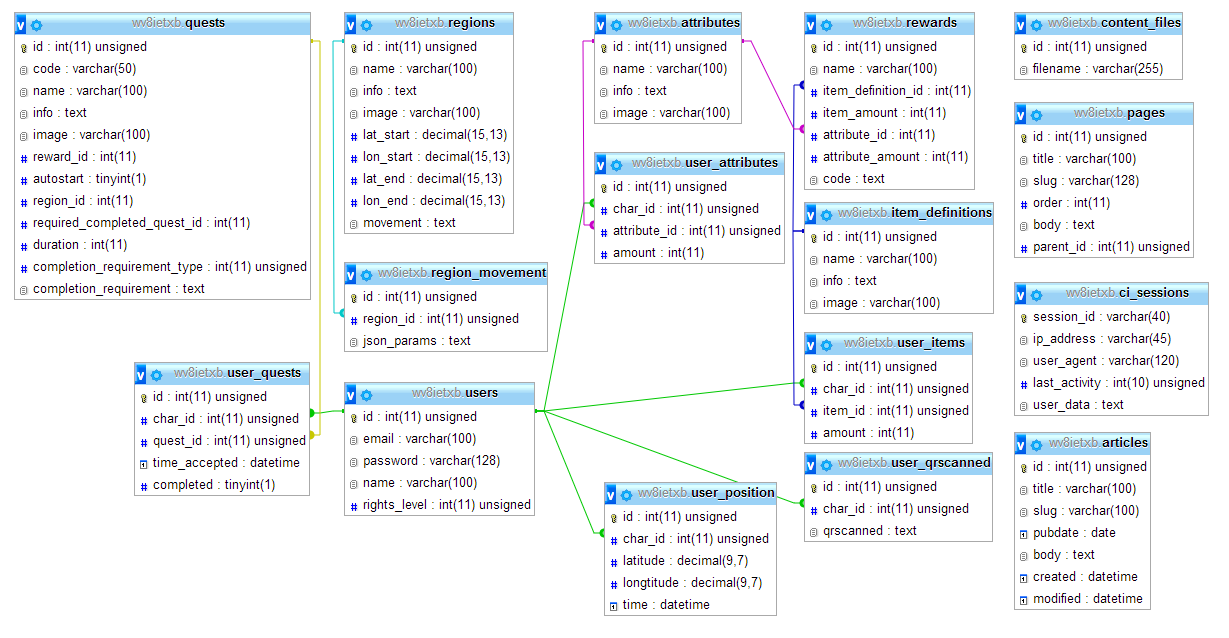
\includegraphics[width=14cm]{mainmatter/imgs/db.png}
  \caption{Tabuľky a ich štruktúra}
  \label{fig:db}
\end{figure}
